%%%%%%%%%%%%%%%%%%%%%%%%%%%%%%%%%%%%%%%%%%%%%%%%%%%%%%%%%%%%%
%% Begin exercise %%
%%%%%%%%%%%%%%%%%%%%%%%%%%%%%%%%%%%%%%%%%%%%%%%%%%%%%%%%%%%%%
\ex{Fundamentals of the magnetic field}


\normalsize{\textbf{Acknowledgement}: The following exercise is adapted from ``Elektrische Maschinen und Antriebe Übungsbuch: Aufgaben mit Lösungsweg'' by A. Binder, Springer, 2017}\\



%%%%%%%%%%%%%%%%%%%%%%%%%%%%%%%%%%%%%%%%%%%%%%%%%%%%%%%%%%%%%
%% Task 1 %%
%%%%%%%%%%%%%%%%%%%%%%%%%%%%%%%%%%%%%%%%%%%%%%%%%%%%%%%%%%%%%

\task{Magnetic iron yoke}
The iron core consists of thin single metal sheets with a cross-sectional area of $A$ = 900 $\si{mm}^2$ and with an air gap of $\delta$ = 3 mm. A simplified sketch is shown in \autoref{fig:MagneticIronCircle}. The material behavior of the selected iron is visualized in \autoref{fig:BH_curve}. The coil with $N$ turns contains a direct current which results in a homogeneous magnetic flux density of $B_{\mathrm{\delta}}$ = 1.8 T in the air gap.


\begin{figure}[htb]
    \centering
    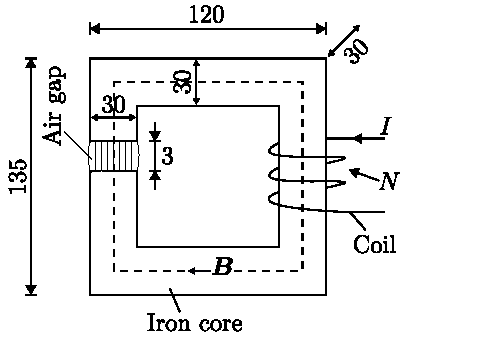
\includegraphics{ex01/MagneticIronCircle.pdf}
    \caption{Simplified sketch of a magnetic iron core. All dimensions of the core are given in mm.}
    \label{fig:MagneticIronCircle}
\end{figure}

\begin{figure}[htb]
    \centering
    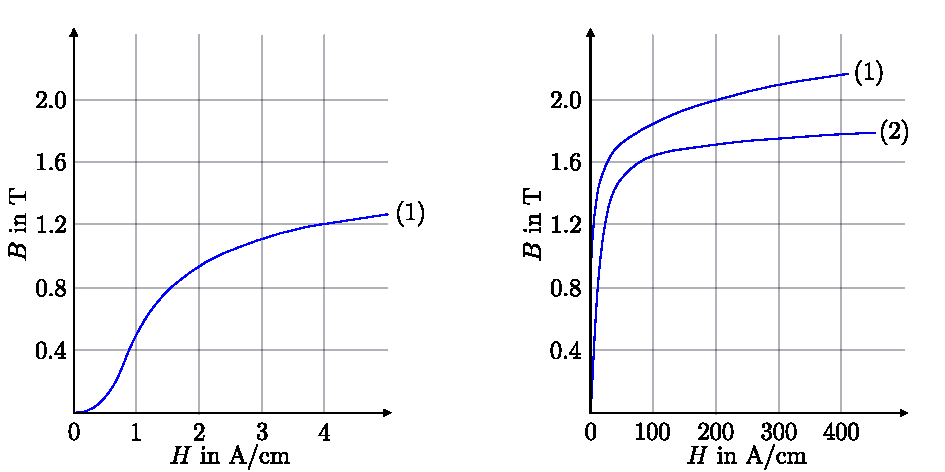
\includegraphics{ex01/BH_curve.pdf}
    \caption{Direct current magnetization curves of electrical steel for (1) hot rolled processing with a thickness of 0.5 mm and (2) cold rolled processing with a thickness of 0.35 mm. The magnetization curve in figure on the left side is a zoomed version of material (1) for lower field strengths.}
    \label{fig:BH_curve}
\end{figure}


%%%%%%%%%%%%%%%%%%%%%%%%%%%%%%%%%%%%%%%%%%%%%%%%%%%%%%%%%%%%%

\subtask{Calculate the magnetic flux $\phi_{\mathrm{\updelta}}$ in the air gap.}
\begin{solutionblock}
    The area of the air gap is equal to the iron core area ($A_{\mathrm{\updelta}} = A = 900 \ \si{mm^2}$).
    The calculation of the magnetic flux is defined as follows:
    \begin{equation}
        \phi_{\updelta} = \int_{S}^{} \boldsymbol{B} \ \mathrm{d} \boldsymbol{S}
        = B A,
    \end{equation}
    where $\boldsymbol{B}$ is the magnetic flux density and $\boldsymbol{S}$ is the surface area to integrate. The above integral could be simplified to B*A because the flux density is homogeneous and the integration surface S  and the flux are perpendicular to each other. 
    This results in
    \begin{equation}
        \phi_{\updelta}  = B_{\updelta} A_{\updelta}
        = 1.8 \ \si{T} \cdot 900 \cdot 10^{-6} \ \si{m^2}
        = 1.62 \ \mathrm{mWb}.
    \end{equation}

\end{solutionblock}



%%%%%%%%%%%%%%%%%%%%%%%%%%%%%%%%%%%%%%%%%%%%%%%%%%%%%%%%%%%%%

\subtask{How big is the magnetic flux density $B_{\mathrm{Fe}}$ in the iron core at the dotted line in \autoref{fig:MagneticIronCircle}? Neglect the leakage flux.}
\begin{solutionblock}
    Since the leakage flux is neglected, the fluxes $\phi_{\mathrm{\updelta}}$ in the air gap and $\phi_{\mathrm{Fe}}$ in the iron are equal. This results in the following equation:
    \begin{equation}
        \phi_{\mathrm{\updelta}} = \phi_{\mathrm{Fe}}
        = A_{\mathrm{\updelta}} B_{\mathrm{\updelta}}
        = A_{\mathrm{Fe}} B_{\mathrm{Fe}}.
    \end{equation}

    The equation from above is resorted to calculate the magnetic flux density:
    \begin{equation}
        B_{\mathrm{Fe}} = B_{\mathrm{\updelta}} \frac{A_{\mathrm{\updelta}}}{A_{\mathrm{Fe}}} = 1.8 \ \si{T}.
    \end{equation}

\end{solutionblock}


%%%%%%%%%%%%%%%%%%%%%%%%%%%%%%%%%%%%%%%%%%%%%%%%%%%%%%%%%%%%%

\subtask{What is the value of the permeability $\mu$ and the magnetic field strengths $H_{\mathrm{\updelta}}$ and $H_{\mathrm{Fe}}$ in the air gap and in the iron for the given operating point?}
\begin{solutionblock}
    The permeability in the air gap is equal to the permeability in the air, which is given with: \newline $\mu = \mu_{\mathrm{0}} = 4 \pi \cdot 10^{-7} \ \frac{\si{Vs}}{\si{Am}}$. The magnetic field strength in the air gap is calculated with:
    \begin{equation}
        H_{\mathrm{\updelta}} = \frac{B_{\mathrm{\updelta}}}{\mu_{\mathrm{0}}}
        = \frac{1.8 \ \si{T}}{4 \pi \cdot 10^{-7} \ \frac{\si{Vs}}{\si{Am}}}
        = 1432395 \ \frac{\si{A}}{\si{m}}.
    \end{equation}

    The curve (1) on the right side in \autoref{fig:BH_curve} shows for $B_{\mathrm{Fe}}$ = 1.8 \si{T} a magnetic filed strength of \newline $H_{\mathrm{Fe}} = 80 \ \frac{\si{A}}{\si{cm}}$ = $8000 \ \frac{\si{A}}{\si{m}}$. With the filed strength $H_{\mathrm{Fe}}$ the permeability of the iron is calculated:
    \begin{equation}
        \mu_{\mathrm{Fe}} = \frac{B_{\mathrm{Fe}}}{H_{\mathrm{Fe}}}
        = \frac{1.8 \ \si{T}}{8000 \ \si{A/m}}
        = 0.000225 \ \frac{\si{Vs}}{\si{Am}},
    \end{equation}
    which is approximately 179 times $\mu_{\mathrm{0}}$.

\end{solutionblock}



%%%%%%%%%%%%%%%%%%%%%%%%%%%%%%%%%%%%%%%%%%%%%%%%%%%%%%%%%%%%%

\subtask{What is the required magnetomotive force $\theta = N \cdot I$ in the excitation coil to excite the flux density $B_{\mathrm{\updelta}}$ = 1.8 T?}
\begin{solutionblock}

    The magnetomotive force is calculated with Ampère's law along closed curve $\partial S$:
    \begin{equation}
        \theta = N I
        = H_{\updelta} \delta + H_{\mathrm{Fe}} l_{\mathrm{Fe}}.
    \end{equation}
    Therefore, the length of the magnetic path calculates as:
    \begin{equation}
        l_{\mathrm{Fe}} = 2(120-30) + 2(135-30)-3 = 387 \ \si{mm}.
    \end{equation}
    Hence, with the two equations from above, the magnetomotive force is calculated with:
    \begin{align}
        \begin{split}
            \theta &= H_{\updelta} \delta + H_{\mathrm{Fe}} l_{\mathrm{Fe}}.\\
            &= 1432395 \ \si{A/m} \cdot 0.003 \ \si{m} + 8000 \ \si{A/m} \cdot 0.387 \ \si{m} \\
            &= 7393 \ \si{A}.
        \end{split}
    \end{align}

\end{solutionblock}



%%%%%%%%%%%%%%%%%%%%%%%%%%%%%%%%%%%%%%%%%%%%%%%%%%%%%%%%%%%%%

\subtask{What is the required current $I$ if the coil has $N$ = 500 turns?}
\begin{solutionblock}
    The current is calculated with:
    \begin{equation}
        I = \frac{\theta}{N} = \frac{7393 \ \si{A}}{500} = 14.79 \ \si{A}.
    \end{equation}

\end{solutionblock}






%%%%%%%%%%%%%%%%%%%%%%%%%%%%%%%%%%%%%%%%%%%%%%%%%%%%%%%%%%%%%
%% Task 2 %%
%%%%%%%%%%%%%%%%%%%%%%%%%%%%%%%%%%%%%%%%%%%%%%%%%%%%%%%%%%%%%


\task{Electromagnetic induction}
A magnetic circuit (cf. \autoref{fig:MagneticIron3D}) has the dimension of $\delta$ = 3 mm, $b$ = $l$ = 30 mm. The excitation coil with $N$ = 500 tuns id fed with an alternating current $i(t) = \hat{I} \sin(2\pi f t)$ with $f$ = 100 Hz and $\hat{I}$ = 7.8 A.
The permeability of the iron $\mu_{\mathrm{Fe}}$ is assumed to be infinite and the flux leakage can be neglected.
A quadratic, non-moving coil with a side length of 30 mm and $N_{\mathrm{C}}$ = 10 turns is within the air gap of the yoke. The orientation of the coil is shown in \autoref{fig:CoilSurface}. 

\begin{figure}[htb]
    \centering
    \begin{subfigure}[b]{0.4\textwidth}
        \centering
        \includegraphics{ex01/MagneticIron3D.pdf}
        \caption{Iron yoke with a coil in the air gap.}
        \label{fig:MagneticIron3D}
    \end{subfigure}
    \quad
    \begin{subfigure}[b]{0.4\textwidth}
        \centering
        \includegraphics{ex01/CoilSurface.pdf}
        \caption{Orientation of the coil surface in the air gap of the given yoke.}
        \label{fig:CoilSurface}
    \end{subfigure}
    \caption{Iron yoke and coil orientation.}
\end{figure}





%%%%%%%%%%%%%%%%%%%%%%%%%%%%%%%%%%%%%%%%%%%%%%%%%%%%%%%%%%%%%

\subtask{Calculate the flux density $B_{\mathrm{\updelta}}(t)$ in the air gap.
Sketch the trajectories of $i(t)$ and $B_{\mathrm{\updelta}}(t)$.}
\begin{solutionblock}

    Since the leakage flux is neglected, the fluxes $\phi_{\mathrm{\updelta}}$ in the air gap and $\phi_{\mathrm{Fe}}$ in the iron are equal ($\phi_{\mathrm{\updelta}} = \phi_{\mathrm{Fe}}$). In addition, the area of the coil and the air gap area are identical ($A_{\mathrm{Fe}} = A_{\mathrm{\updelta}}$).
    Therefore, the following relationship is made:
    \begin{equation}
        \phi_{\mathrm{\updelta}} = \phi_{\mathrm{Fe}}
        = A_{\mathrm{\updelta}} B_{\mathrm{\updelta}}
        = A_{\mathrm{Fe}} B_{\mathrm{Fe}}.
    \end{equation}
    By resorting the equation from above, the flux density in the air gap is calculated:
    \begin{equation}
        B_{\mathrm{Fe}} = B_{\mathrm{\updelta}} \frac{A_{\mathrm{\updelta}}}{A_{\mathrm{Fe}}} = B_{\mathrm{\updelta}}.
    \end{equation}
    
    The magnetic field strength calculates as:
    \begin{equation}
        H_{\mathrm{Fe}} = \frac{B_{\mathrm{Fe}}}{\mu_{\mathrm{Fe}}} = 0,
    \end{equation}
    which is zero due to the assumption of an infinite permeability in the iron path.

    In the following equation, Ampère's law is given with:
    \begin{equation}
        \theta(t) = N i(t)
        = H_{\mathrm{\updelta}} \delta + H_{\mathrm{Fe}} l_{\mathrm{Fe}}.
    \end{equation}
        
    This equation simplifies by neglecting the magnetic field strength within the iron ($H_{\mathrm{Fe}}$ = 0) due to the infinite permeability. This leads to the following equation:
    \begin{equation}
        \theta(t) = H_{\mathrm{\updelta}} \delta
        = \frac{B_{\mathrm{\updelta}} \delta}{\mu_{\mathrm{0}}},
    \end{equation}
    where $H_{\updelta}$ = $B_{\updelta} \ / \ \mu_{\mathrm{0}}$.

    By rearranging the equation from above, the magnetic flux density in the air gap is calculated as follows:
    \begin{equation}
        B_{\mathrm{\updelta}}(t) = \frac{\mu_{\mathrm{0}} N i(t)}{\delta}.
    \end{equation}
    
    With the given values in the task, the time course of the magnetic flux density is expressed as:
    \begin{equation}
        B_{\mathrm{\updelta}}(t) = 4 \pi \cdot 10^{-7} \cdot \frac{500 \cdot 7.8 \ \si{A} \cdot \sin(2 \pi \cdot 100 \ \si{Hz} \cdot t)}{0.003 \ \si{m}}
        = 1.63 \ \si{T} \cdot \sin(2 \pi \cdot 100 \ \si{Hz} \cdot t).
    \end{equation}

    In the upper part of \autoref{fig:solution_FluxDensity} the trajectory of the current is shown. In addition, the trajectory of the magnetic flux density is visualized in the lower part.
    \begin{solutionfigure}[ht]
        \centering
        \includegraphics{ex01/solution_FluxDensity.pdf}
        \caption{Trajectories of the current $i(t)$ in the upper and the magnetic flux density $B(t)$ in the lower part of the figure.}
        \label{fig:solution_FluxDensity}
    \end{solutionfigure}

\end{solutionblock}



%%%%%%%%%%%%%%%%%%%%%%%%%%%%%%%%%%%%%%%%%%%%%%%%%%%%%%%%%%%%%

\subtask{How large is the magnetic flux linkage $\mathit{\Psi}(t)$ of the magnetic field generated by the excitation coil to the coil in the air gap?}
\begin{solutionblock}

    According to \autoref{fig:CoilSurface}, the direction of vector d$\boldsymbol{S}$ is in the opposite direction of the flux density vector $\boldsymbol{{B}}_{\updelta}$. Therefore, the flux linkage has a negative sign:
    \begin{equation}
        \psi(t) = N_{\mathrm{c}} \phi(t)
        = - N_{\mathrm{c}} A_{\mathrm{\updelta}} B_{\mathrm{\updelta}}(t).
    \end{equation}

    With the given and calculated values, the flux linkage is defined with:
    \begin{equation}
        \psi(t) = -10 \cdot (30 \cdot 30) \cdot 10^{-6} \ \si{m^2} \cdot 1.63 \ \si{T} \cdot \sin(2 \pi  \cdot 100 \ \si{Hz} \cdot t)
        = -0.0147 \ \si{Vs} \cdot \sin(2 \pi \cdot 100 \ \si{Hz} \cdot t).
    \end{equation}

\end{solutionblock}


%%%%%%%%%%%%%%%%%%%%%%%%%%%%%%%%%%%%%%%%%%%%%%%%%%%%%%%%%%%%%

\subtask{How large is the induced voltage $u_{\mathrm{i}}(t)$ of the coil in the air gap? Also, sketch the trajectory $u_{\mathrm{i}}$.}
\begin{solutionblock}
    The induced voltage is the differential of the magnetic flux linkage and therefore, defined as:
    \begin{equation}
        u_{\mathrm{i}}(t) = -\frac{\mathrm{d}\psi(t)}{\mathrm{d}t}
        = - 2 \pi f \mathit{\hat{\Psi}} \cos(2 \pi f t).
    \end{equation}

    In addition, the induced voltage is calculated with the previous calculated values:
    \begin{equation}
        u_{\mathrm{i}}(t) = -2 \pi \cdot 100 \ \si{Hz} \cdot (-0.0147 \ \si{Vs}) \cdot \cos(2 \pi \cdot 100 \ \si{Hz} \cdot t)
        = 9.2 \ \si{V} \cdot \cos(2 \pi \cdot 100 \ \si{Hz} \cdot t).
    \end{equation}

    In the upper part of \autoref{fig:solution_InducedVoltage}, the calculated current from the previous task is shown again. The induced voltage is visualized in the lower part of the figure. 
    \begin{solutionfigure}[ht]
        \centering
        \includegraphics{ex01/solution_InducedVoltage.pdf}
        \caption{Trajectories of the current $i(t)$ in the upper and the induced voltage $u_{\mathrm{i}}(t)$ in the lower part of the figure.}
        \label{fig:solution_InducedVoltage}
    \end{solutionfigure}
    
\end{solutionblock}



%%%%%%%%%%%%%%%%%%%%%%%%%%%%%%%%%%%%%%%%%%%%%%%%%%%%%%%%%%%%%

\subtask{Calculate the mutual inductance $M$ between the excitation coil and the air gap coil.}
\begin{solutionblock}
   The mutual inductance is defined as follows:
    \begin{equation}
        M = M_{\mathrm{21}} = \frac{\psi_{\mathrm{2}}(t)}{i_{\mathrm{1}}(t)}
        = \frac{\mathit{\hat{\Psi}} \sin(2 \pi f t)}{\hat{I} \sin(2 \pi f t)}
        = \frac{\mathit{\hat{\Psi}}}{\hat{I}}
        = \frac{-0.0147 \ \si{Vs}}{7.8 \ \si{A}}
        = -1.88 \ \si{mH}.
    \end{equation}

\end{solutionblock}





%%%%%%%%%%%%%%%%%%%%%%%%%%%%%%%%%%%%%%%%%%%%%%%%%%%%%%%%%%%%%
%% Task 3 %%
%%%%%%%%%%%%%%%%%%%%%%%%%%%%%%%%%%%%%%%%%%%%%%%%%%%%%%%%%%%%%


\task{Moving current-carrying conductor in a magnetic field}
An electrical conductor (length $l$ = 1 m, resistance $R$ = 0.2 $\Omega$) is connected via two flexible supply lines from a battery (open circuit voltage $U_{\mathrm{B0}}$ = 12 V, internal resistance $R_{\mathrm{Bi}}$ = 0.1 $\Omega$) and is excited with direct current $I$. The conductor is located in an air gap between two very long permanent magnets pole pieces, that are perpendicular to the conductor axis.
The magnetic flux density directed downwards perpendicular to the conductor axis $B_{\mathrm{\updelta}}$ = 0.8 T in the air gap. The self-inductance of the conductor and the wire connections is neglected.

\begin{figure}[htb]
    \centering
    \includegraphics{ex01/ConductorInMagneticField.pdf}
    \caption{Current-carrying conductor in magnetic field.}
    \label{fig:ConductorInMagneticField}
\end{figure}


%%%%%%%%%%%%%%%%%%%%%%%%%%%%%%%%%%%%%%%%%%%%%%%%%%%%%%%%%%%%%

\subtask{Draw the electrical equivalent circuit diagram of the battery and resting conductor, and enter the direction of current flow $I$ in the load convention style. How large is $I$?}
\begin{solutionblock}
    As the magnetic field is constant over time, no induction occurs. Only the electrical battery voltage acts according to the equivalent circuit diagram in \autoref{fig:solution_EquivalentCircuitDiagram}. Hence, the current is calculated with:
    \begin{equation}
        I = \frac{U_{\mathrm{B0}}}{R_{\mathrm{Bi}}+R}
        = \frac{12 \ \si{V}}{(0.1+0.2) \ \si{\Omega}}
        = 40 \ \si{A}.
    \end{equation}

    \begin{solutionfigure}[ht]
        \centering
        \includegraphics{ex01/solution_equivalentCircuitDiagram.pdf}
        \caption{Equivalent circuit diagram for the battery and resting conductor marked here with $R$.}
        \label{fig:solution_EquivalentCircuitDiagram}
    \end{solutionfigure}

\end{solutionblock}



%%%%%%%%%%%%%%%%%%%%%%%%%%%%%%%%%%%%%%%%%%%%%%%%%%%%%%%%%%%%%

\subtask{In which direction shows the Lorentz force $F$ on the conductor? How big is this force?}
\begin{solutionblock}
    The force $F$ acts at right angles to the field and current flow direction, this means, in the direction of the air gap surface to the right, which is shown in \autoref{fig:solution_LorentzForce}. Since the direction of current flow and field direction form a right angle with each other, the maximum possible force occurs:
    \begin{equation}
        F = I l B_{\mathrm{\updelta}}
        = 40 \ \si{A} \cdot 1 \ \si{m} \cdot 0.8 \ \si{T}
        = 32 \ \si{N}.
    \end{equation}
    
    As the conductor is flexibly connected to the battery via flexible connections the force $F$ in the air gap accelerates it to the right in its direction.

    \begin{solutionfigure}[ht]
        \centering
        \includegraphics{ex01/solution_LorentzForce.pdf}
        \caption{Acting Lorentz force on the conductor in the air gap.}
        \label{fig:solution_LorentzForce}
    \end{solutionfigure}

\end{solutionblock}



%%%%%%%%%%%%%%%%%%%%%%%%%%%%%%%%%%%%%%%%%%%%%%%%%%%%%%%%%%%%%

\subtask{Draw the electrical equivalent circuit diagram for the combination of the moving conductor and feeding battery with the conditions at conductor side $l$. What additional electrical voltage occurs?}
\begin{solutionblock}
    If the conductor is moved by the force $F$ at the speed $v$, the movement induction in the conductor along the length $l$ creates a movement field strength against the direction of the tangent vector:
    \begin{equation}
        \boldsymbol{E}_{\mathrm{b}} = \boldsymbol{v} \times \boldsymbol{B}_{\mathrm{\updelta}}.
    \end{equation}
    
    Therefore, between 2 and 1 the voltage $u_{\mathrm{i}}$ is induced:
    \begin{equation}
        u_{\mathrm{i}}
        = \int_{2}^{1} (\boldsymbol{v} \times \boldsymbol{B}_{\updelta}) \mathrm{d}\boldsymbol{s}
        = - \int_{2}^{1} v B_{\updelta} \mathrm{d}s
        = -v B_{\updelta} l
        = U_{\mathrm{i}}.
    \end{equation}

    In the equivalent circuit diagram (\autoref{fig:solution_movingConductor}), the induced voltage acts in series with the battery voltage:
    \begin{equation}
        U_{\mathrm{B0}} + U_{\mathrm{i}} = (R_{\mathrm{Bi}} + R) I
        = U_{\mathrm{B0}} - v B_{\updelta} l.
    \end{equation}

    As long as $v B_{\updelta} l$ is less than $U_{\mathrm{B0}}$, is $I$ > 0 and the driving force $F$ > 0 remains effective. The induced voltage acts against the current direction $I$, which is the cause of the conductor movement through $F$, and therefore acts against the cause of its creation (Lenz's rule, \autoref{fig:solution_movingConductor}).

    \begin{solutionfigure}[ht]
        \centering
        \includegraphics{ex01/solution_movingConductor.pdf}
        \caption{Moving conductor with the induced voltage $u_{\mathrm{i}}$ as an external voltage, a) equivalent electrical circuit diagram, b) direction of the Lorentz force $F$.}
        \label{fig:solution_movingConductor}
    \end{solutionfigure}

\end{solutionblock}




%%%%%%%%%%%%%%%%%%%%%%%%%%%%%%%%%%%%%%%%%%%%%%%%%%%%%%%%%%%%%

\subtask{To what final velocity $v_{\mathrm{0}}$ is the conductor in the air gap accelerated by $F$ if no mechanical braking force acts on it and if one considers the air gap as arbitrary long? How is the current $I$ in the conductor after reaching the final velocity?}
\begin{solutionblock}

    The final velocity $v_{\mathrm{0}}$ in the air gap is reached when, the sum of all forces acting on the conductor is zero ($\sum F = 0$), according to Newton's second axiom.
    Without mechanical forces from outside, this is this only true when $I$ = 0 due to $F = I l B_{\updelta}$. With the equivalent circuit from \autoref{fig:solution_movingConductor} the following equation is defined:
    \begin{equation}
        U_{\mathrm{B0}} = (R_{\mathrm{Bi}} + R) I - U_{\mathrm{i}},
    \end{equation}
    with $I$ = 0, it arranges to:
    \begin{equation}
        U_{\mathrm{B0}} = - U_{\mathrm{i}}
        = v_{\mathrm{0}} B_{\updelta} l.
    \end{equation}

    Hence, the final velocity is calculated as:
    \begin{equation}
        v_{\mathrm{0}} = \frac{U_{\mathrm{B0}}}{B_{\updelta} l}
        = \frac{12 \ \si{V}}{0.8 \ \si{T} \cdot 1 \ \si{m}}
        = 15 \ \frac{\si{m}}{\si{s}}.
    \end{equation}

    At the final speed $v_{\mathrm{0}}$, the induced voltage and battery voltage canceled each other out, such that the current $I$ is zero.

\end{solutionblock}


%%%%%%%%%%%%%%%%%%%%%%%%%%%%%%%%%%%%%%%%%%%%%%%%%%%%%%%%%%%%%

\subtask{Assume that the conductor experiences a braking force due to friction $F_{\mathrm{R}}$= 10 N. To what final velocity $v$ does the conductor now accelerate? What is the current $I$ in the conductor?}
\begin{solutionblock}
    The final velocity $v$ is reached when no further accelerating force acts on the conductor, i.e., when $F - F_{\mathrm{R}} = 0$. The force $F$ is defined as:
    \begin{equation}
        F = I l B_{\updelta}
        = F_{\mathrm{R}} = 10 \ \si{N}.
    \end{equation}
    By rearranging, the necessary current is calculated with:
    \begin{equation}
        I = \frac{10 \ \si{N}}{1 \ \si{m} \cdot 0.8 \ \si{T}}
        = 12.5 \ \si{A}.
    \end{equation}

    With the voltage equation again from the equivalent circuit diagram:
    \begin{equation}
        U_{\mathrm{B0}} = (R_{\mathrm{Bi}}+R)I - u_{\mathrm{i}},
    \end{equation}
    with
    \begin{equation}
        u_{\mathrm{i}} = - v B_{\updelta} l.
    \end{equation}
    Hence, the velocity $v$ calculates as follows:
    \begin{equation}
        v = \frac{U_{\mathrm{B0}}-(R_{\mathrm{Bi}}+R)I}{B_{\updelta} l}
        = \frac{12 \ \si{V} - 0.3 \ \si{\Omega} \cdot 12.5 \ \si{A}}{0.8 \ \si{T} \cdot 1 \ \si{m}}
        = 10.31 \ \frac{\si{m}}{\si{s}}.
    \end{equation}

    The Lorentz force and the friction force are visualized in \autoref{fig:solution_LorentzForce_balanceOfForces} after reaching the final speed.
    \begin{solutionfigure}[ht]
        \centering
        \includegraphics{ex01/solution_LorentzForce_balanceOfForces.pdf}
        \caption{Indicates the balance of forces after reaching the final speed.}
        \label{fig:solution_LorentzForce_balanceOfForces}
    \end{solutionfigure}

\end{solutionblock}



%%%%%%%%%%%%%%%%%%%%%%%%%%%%%%%%%%%%%%%%%%%%%%%%%%%%%%%%%%%%%

\subtask{What mechanical power $P_{\mathrm{m}}$ is required so that the conductor can move against the braking friction force $F_{\mathrm{R}}$ = 10 N with the final velocity $v$ determined in task 3.5. Sketch the curves $v(I)$ and $v(F)$ for a variable braking force $F_{\mathrm{R}}$ between $v_{\mathrm{0}}$ and $v$ = 0.}
\begin{solutionblock}

    The mechanical power is calculated as follows:
    \begin{equation}
        P_{\mathrm{m}} = F_{\mathrm{R}} v
        = 10 \ \si{N} \cdot 10.31 \ \si{m/s}
        = 103.1 \ \si{W}.
    \end{equation}

    The relationship between the current and the velocity is calculated with:
    \begin{equation}
        v = \frac{U_{\mathrm{B0}}-(R_{\mathrm{Bi}}+R)I}{B_{\updelta} l},
    \end{equation}
    by changing the value of the current. This results in the left part of \autoref{fig:solution_conductorSpeed}.
    The corresponding force $F$ is calculated as:
    \begin{equation}
        F = I l B_{\updelta},
    \end{equation}
    and the resulting values are shown in der right part of \autoref{fig:solution_conductorSpeed}.
    \begin{solutionfigure}[ht]
        \centering
        \includegraphics{ex01/solution_conductorSpeed.pdf}
        \caption{Current and force of the conductor in relationship to the velocity.}
        \label{fig:solution_conductorSpeed}
    \end{solutionfigure}

\end{solutionblock}



%%%%%%%%%%%%%%%%%%%%%%%%%%%%%%%%%%%%%%%%%%%%%%%%%%%%%%%%%%%%%

\subtask{What is the electrical power drawn from the battery $P_{\mathrm{el}}$ for the operating point from task 3.5? What is the efficiency $\eta$ and the power loss $P_{\mathrm{l}}$ when converting electrical power into mechanical power? How does the conductor act as an electromechanical energy converter?}
\begin{solutionblock}
    The electrical power for the given operating point is calculated with:
    \begin{equation}
        P_{\mathrm{el}} = U_{\mathrm{B0}} I
        = 12 \ \si{V} \cdot 12.5 \ \si{A}
        = 150 \ \si{W},
    \end{equation}
    which is used in the next step for the efficiency calculation:
    \begin{equation}
        \eta = \frac{P_{\mathrm{out}}}{P_{\mathrm{in}}}
        = \frac{P_{\mathrm{m}}}{P_{\mathrm{el}}}
        = \frac{103.1 \ \si{W}}{150 \ \si{W}}
        = 68.7 \ \si{\%}.
    \end{equation}

    The total losses are calculated as follows:
    \begin{equation}
        P_{\mathrm{l}} = P_{\mathrm{in}} - P_{\mathrm{out}}
        = 150 \ \si{W} - 103.1 \ \si{W}
        = 46.9 \ \si{W}.
    \end{equation}

    The conductor moves against the braking external frictional force $F_{\mathrm{R}}$, hence, it acts as a motor. It converts electrical energy from the battery into mechanical energy.

\end{solutionblock}

